\documentclass[handout]{beamer} 
\title{ITCS 532:\\ W3 Homework Solutions}
\date{}
\author{Rob Egrot}

\usepackage{amsmath, bbold, bussproofs,graphicx}
\usepackage{mathrsfs}
\usepackage{amsthm}
\usepackage{amssymb}
\usepackage[all]{xy}
\usepackage{multirow}
\usepackage{tikz-cd}


\newtheorem{proposition}[theorem]{Proposition}
\newcommand{\bN}{\mathbb{N}}
\newcommand{\bZ}{\mathbb{Z}}
\newcommand{\bQ}{\mathbb{Q}}
\newcommand{\bR}{\mathbb{R}}
\newcommand{\bP}{\mathbb{P}}
\newcommand{\tvs}{\textvisiblespace}
\newcommand{\ra}{\rightarrow}
\newcommand{\la}{\leftarrow}
\newcommand{\co}{\mathbf{code}}

\addtobeamertemplate{navigation symbols}{}{%
    \usebeamerfont{footline}%
    \usebeamercolor[fg]{footline}%
    \hspace{1em}%
    \insertframenumber/\inserttotalframenumber
}
\setbeamertemplate{theorems}[numbered]
\begin{document}

\begin{frame}
\titlepage
\end{frame}

\begin{frame}
\frametitle{Q1}
What does this machine do?

\begin{center}
\begin{tikzpicture}[scale=0.15]
\tikzstyle{every node}+=[inner sep=0pt]
\draw [black] (9.4,-31.3) circle (3);
\draw (9.4,-31.3) node {$q_0$};
\draw [black] (22.4,-31.3) circle (3);
\draw (22.4,-31.3) node {$q_1$};
\draw [black] (36,-31.6) circle (3);
\draw (36,-31.6) node {$q_2$};
\draw [black] (22.4,-44.4) circle (3);
\draw (22.4,-44.4) node {$q_3$};
\draw [black] (22.4,-44.4) circle (2.4);
\draw [black] (22.4,-16.2) circle (3);
\draw (22.4,-16.2) node {$q_4$};
\draw [black] (22.4,-16.2) circle (2.4);
\draw [black] (12.4,-31.3) -- (19.4,-31.3);
\fill [black] (19.4,-31.3) -- (18.6,-30.8) -- (18.6,-31.8);
\draw (15.9,-31.8) node [below] {$:,\ra$};
\draw [black] (11.36,-29.03) -- (20.44,-18.47);
\fill [black] (20.44,-18.47) -- (19.54,-18.75) -- (20.3,-19.41);
\draw (15.35,-22.3) node [left] {$\{a,\tvs\},\tvs$};
\draw [black] (33.284,-32.856) arc (-72.05443:-110.47292:12.503);
\fill [black] (33.28,-32.86) -- (32.37,-32.63) -- (32.68,-33.58);
\draw (29.13,-34.02) node [below] {$a,\tvs$};
\draw [black] (24.914,-29.684) arc (114.19527:63.27739:10.059);
\fill [black] (24.91,-29.68) -- (25.85,-29.81) -- (25.44,-28.9);
\draw (29.29,-28.23) node [above] {$\tvs,\ra$};
\draw [black] (22.4,-34.3) -- (22.4,-41.4);
\fill [black] (22.4,-41.4) -- (22.9,-40.6) -- (21.9,-40.6);
\draw (21.9,-37.85) node [left] {$\tvs,\tvs$};
\draw [black] (34.01,-29.35) -- (24.39,-18.45);
\fill [black] (24.39,-18.45) -- (24.54,-19.38) -- (25.29,-18.72);
\draw (29.74,-22.45) node [right] {$\{:,a\},\ra$};
\draw [black] (22.4,-28.3) -- (22.4,-19.2);
\fill [black] (22.4,-19.2) -- (21.9,-20) -- (22.9,-20);
\draw (22.9,-23.75) node [right] {$:,\ra$};
\end{tikzpicture}
\end{center}

Erases its input.
\end{frame}

\begin{frame}
\frametitle{Q2}
Write out the transition function $\delta$ for $T$ from Q1 in terms of tuples (i.e. $(q,\sigma,q',\sigma'))$. Since $\sigma_0$, $\sigma_1$, $\sigma_2$, and $\sigma_3$ are taken by $:$, $\tvs$, $\la$ and $\ra$ respectively we let $a=\sigma_4$.
\begin{itemize}
\item $(q_0, :, q_1, \ra) = (q_0,\sigma_0,q_1,\sigma_3)$.
\item $(q_0, \tvs, q_4, \tvs) = (q_0,\sigma_1,q_4,\sigma_1)$.
\item $(q_0,a,q_4,\tvs) = (q_0, \sigma_4,q_4,\sigma_1)$.
\item $(q_1, :, q_4, \ra)= (q_1,\sigma_0,q_4,\sigma_3)$.
\item $(q_1,\tvs,q_3,\tvs) = (q_1,\sigma_1,q_3,\sigma_1)$.
\item $(q_1,a,q_2,\tvs) = (q_1,\sigma_4,q_2,\sigma_1)$.
\item $(q_2,:,q_4,\ra) = (q_2,\sigma_0,q_4,\sigma_3)$.
\item $(q_2,\tvs,q_1,\ra) = (q_2,\sigma_1,q_1,\sigma_3)$.
\item $(q_2,a,q_4,\ra) = (q_2,\sigma_4, q_4,\sigma_3)$.
\end{itemize}


\end{frame}

\begin{frame}
\frametitle{Q3}
Using the system from the notes and your transition function from Q2 write down $\co(T)$.
 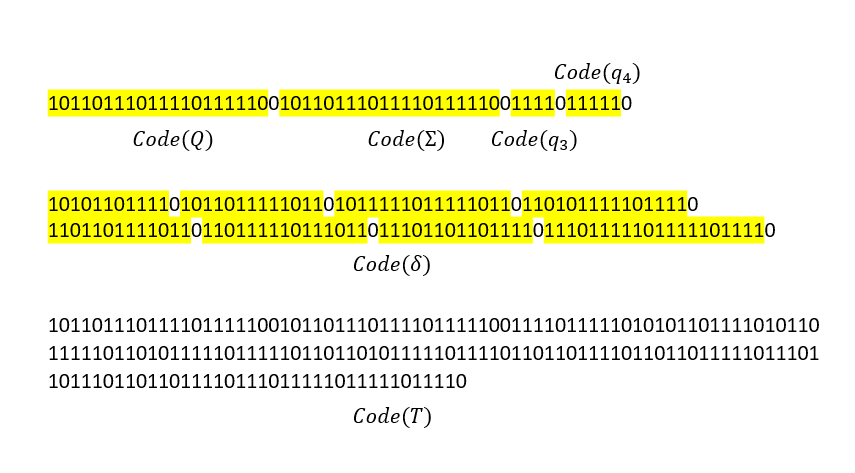
\includegraphics[width=\linewidth]{code.png}
\end{frame}

\begin{frame}
\frametitle{Q4}
Suppose $T$ is a Turing machine over the alphabet $\{0,1,*\}$ that takes as input two binary numbers separated by $*$ and outputs their sum (in binary). Describe a way we could use $T$ to construct a Turing machine that takes as input two positive binary numbers separated by $*$ and outputs their product.
\begin{enumerate}
\item Copy first number to tape 2.
\item Copy second number to tape 3. 
\item Trim tape 1 so it just contains first number.
\item If tape 3 is empty then erase tape 1 and halt.
\item If the number on tape 3 is one then halt.
\item Add number on tape 2 to the number on tape 1, then decrease number on tape 3 by one (we use $T$ in this step).
\item Go to step 5).
\end{enumerate}
\end{frame}



\end{document}